\documentclass{VUMIFPSbakalaurinis}
\usepackage{algorithmicx}
\usepackage{algorithm}
\usepackage{algpseudocode}
\usepackage{amsfonts}
\usepackage{amsmath}
\usepackage{bm}
\usepackage{caption}
\usepackage{color}
\usepackage{float}
\usepackage{graphicx}
\usepackage{listings}
\usepackage{subfig}
\usepackage{wrapfig}
\usepackage{tabularx}
\usepackage{multirow}
\usepackage{enumitem}
\usepackage{graphicx}

%PAKEISTA, tarpai tarp sąrašo elementų
\setitemize{noitemsep,parsep=0.7pt,partopsep=0.7pt}
\setenumerate{noitemsep,parsep=0.7pt,partopsep=0.7pt}

% Titulinio aprašas
\university{Vilniaus universitetas}
\faculty{Matematikos ir informatikos fakultetas}
\department{Programų sistemų katedra}
\papertype{Bakalauro darbas}
\title{Skaitmeninės tapatybės valdymas taikant blokų grandinę}
\titleineng{Digital Identity Management using Blockchain}
\author{Jurgis Kargaudas}
% \secondauthor{Vardonis Pavardonis}   % Pridėti antrą autorių
\supervisor{asist. Aurimas Šimkus}
\reviewer{TO BE ADDED}
\date{Vilnius – \the\year}

% Nustatymai
% \setmainfont{Palemonas}   % Pakeisti teksto šriftą į Palemonas (turi būti įdiegtas sistemoje)
\bibliography{Bakalaurinis}

\begin{document}
\maketitle

%% Padėkų skyrius
% \sectionnonumnocontent{}
% \vspace{7cm}
% \begin{center}
%     Padėkos asmenims ir/ar organizacijoms
% \end{center}

\sectionnonumnocontent{Santrauka}

Šiame darbe nagrinėtas blokų grandinės technologijos tinkamumas skaitmeninės tapatybės valdyme. Pristačius naudotojų poreikius identiteto valdymui internete,
apžvelgtas esamų modelių gebėjimas juos išpildyti. Apibendrinus liekančias naudotojų problemas, tirta blokų grandinė ir jos charakteristikos,
kurios leistų įveikti kylančius iššūkius skaitmeninės tapatybės valdyme.

Nustatyta, kad blokų grandinė gali būti taikoma skaitmeninės tapatybės valdymui internete. Pristatytas blokų grandine ir išmaniaisias kontraktais
paremtas atributų valdymo modelis,
leidžiantis naudotojams kontroliuoti savo asmens duomenis ir jų sklaidą. Sukurtas pateikto modelio prototipas, parašytas su \enquote{Solidity}
programavimo kalba.

\raktiniaizodziai{skaitmeninė tapatybė, skaitmeninės tapatybės valdymas, blokų grandinė, išmanieji kontraktai.}   

% English version

\sectionnonumnocontent{Summary}
In this paper, blockchain applicability for digital identity management was investigated. After presenting user needs for identity management,
currently used identity management models were researched. Following that, blockchain and its characteristics were examined,
in order to find out whether the technology is suitable
to overcome present user identification challenges.

It was determined that blockchain can be used for digital identity management in the internet. A blockchain and smart contract based attribute management model was presented,
which allows users to take control of their own personal data and it's distribution. A prototype of the model was presented,
which was written in \enquote{Solidity} programming language.

\keywords{digital identity, digital identity management, blockchain, smart contracts.}

\sectionnonum{Įvadas}
Interneto paslaugos šiais laikais yra neatsiejama žmonių gyvenimo dalis.
Norėdami individualizuoti turinį, sustiprinti taikomosios programos saugumą ar siekdami
iš anksto išvengti kenkėjiškų tikslų turinčių asmenų ar sukurtų robotų, paslaugų tiekėjai
siekia identifikuoti savo naudotojus. Interneto naudotojų skaičiui perkopus 4 milijardus \cite{InternetUsers2018},
o kiekvienam naudotojui vidutiniškai turint po 7 skirtingas socialines paskyras \cite{Mander2017}, asmenų
tapatybių valdymas, autentifikavimas ir autorizavimas tampa vis didesniu iššūkiu.

Tapatybių valdymas kelia problemų tiek paslaugų tiekėjams, tiek jų naudotojams. Kiekvienas
paslaugų tiekėjas turi skirti papildomų resursų naudotojų tapatybių valdymui, jų autentifikavimui,
jautrių duomenų saugumo užtikrinimui. Paslaugų naudotojams bene didžiausi atsiradę keblumai:
milžiniškas įsimintinų slaptažodžių kiekis bei sunkumai kontroliuojant savo asmens duomenų sklaidą
skirtingose sistemose. Vidutiniškai interneto naudotojas turi 25 slaptažodžių reikalaujančias paskyras
ir per dieną turi įvesti 8-is slaptažodžius \cite{Florencio2007}. Susidarius tokiai situacijai, per didelis įsimintinų slaptažodžių kiekis neretai 
priverčia naudotojus paaukoti saugumą dėl patogumo
ir pradėti naudoti tą patį slaptažodį sirtingoms sistemoms \cite{Pashalidis2003, Samar1999}. Naudotojas, turėdamas keletą
paskyrų skirtingose sistemose, taip pat praranda dalį savo asmens duomenų kontrolės. Jam tenka pasitikėti
taikomosios programos naudojamomis technologijomis ir metodais ir tikėtis, kad jie bus pakankamai saugūs
ir stabilūs bei suteikti asmens duomenys nepasieks nepageidaujamų adresatų. Didėjant naudojamų paslaugų kiekiui,
naudotojo skaitmeninės tapatybės duomenis turi vis daugiau taikomųjų programų ir bent vienai iš jų
patyrus programišių įsilaužimą ar kitokią nesėkmę, jautrūs naudotojo duomenys būna paviešinti. 

Vienu iš pagrindinių skaitmeninės tapatybės valdymo keliamų problemų sprendimu išlieka vienkartinis prisijungimas
 (angl. \textit{Single Sign-On}). Šis sprendimas leidžia naudotojui pasirinkti
vieną tapatybės tiekėją (angl. \textit{identity provider}) ir patikėti jam skaitmeninės tapatybės valdymą. Tuomet naudotojas prie visų
paslaugų, palaikančių pasirinkto tapatybės tiekėjo (pvz. \textit{Facebook}) prisijungimą, gali autentifikuotis naudodamas ta pačia paskyra. Tokiu
būdu naudotojui pakanka prisiminti tik slaptažodžius, užregistruotus tapatybės tiekėjų sistemose, o paslaugų
tiekėjai neturi patys rūpintis autentifikavimu ar autorizavimu, o jį užtikrina integruodami sistemą
su tapatybės tiekėju. Tačiau šis sprendimo būdas taip pat turi aiškių trūkumų: naudotojas negali prisijungti
prie paslaugų, nepalaikančių pasirinkto tapatybės tiekėjo, dėl paslaugų tiekėjų priklausomybės nuo tapatybės tiekėjo pastarojo pasiekiamumas
tampa vieninteliu nesėkmės tašku (angl. \textit{single point of failure}), naudotojas taip pat praranda dalį savo asmens duomenų kontrolės.
Naršantis internete asmuo yra priverstas pasitikėti tapatybės tiekėjo
gebėjimu perduoti tik naudotojo leistus asmens duomenis ir tik toms trečiosioms šalims, kurias jis patvirtina.
Kaip rodo \textit{Cambridge Analytica} incidentas \cite{CambridgeAnalytica}, net didžiosios kompanijos, tokios
kaip \textit{Facebook}, ne visada sugeba tai užtikrinti.

Blokų grandinė (angl. \textit{blockchain}) yra nauja alternatyva skaitmeninės tapatybės valdymui. Ši technologija veikia kaip
paskirstytų įrašų platforma (angl. \textit{distributed ledger platform}), kurioje kiekvienas įrašas yra nekintamas (angl. \textit{immutable}), o visi
užfiksuoti įrašai atspindi tikslią transakcijų istoriją nuo pat grandinės sukūrimo \cite{Baars2016}. Saugant tapatybės duomenis šioje grandinėje ir
pritaikius reikiamą blokų grandinės pasiekiamumo lygį įrašų rašymui ir skaitymui, asmuo visada
žino, kokia trečioji šalis gali pasiekti kokius tapatybės duomenis. Kadangi blokų grandinė yra decentralizuota, pritaikius ją skaitmeninių tapatybių valdyme taip pat
būtų galima išvengti šioje srityje dažnos vienintelio nesėkmės taško problemos. Šiame darbe nagrinėjama, kada verta naudoti blokų grandinę
naudotojų skaitmeniniam autentifikavimui bei autorizavimui, kokie to pranašumai, trūkumai bei priėmimo barjerai (angl. \textit{adoption barriers}).
\\

\textbf{Darbo tikslas} - išanalizuoti blokų grandinės tinkamumą skaitmeninės tapatybės valdymui.
\\

\textbf{Darbe keliami uždaviniai}:

\begin{enumerate}
    \item Išnagrinėti esamus skaitmeninės tapatybės valdymo sprendimus ir jų keliamus iššūkius.
    \item Apibūdinti blokų grandines ir jų savybes, leidžiančias spręsti dabartines identifikavimo problemas.
    \item \textit{Apžvelgti esamas blokų grandinės sistemas, taikomas naudotojų autentifikavimui ar autorizavimui}.
    \item Pateikti blokų grandinės panaudos atvejį skaitmeninės tapatybės valdymui ir sukurti jo veikimą demonstruojantį prototipą.
    \item Įvertinti pateikto sprendimo tinkamumą apibūdinant jo privalumus, trūkumus ir pritaikymo barjerus.
    \item Palyginti pristatytą sprendimą su standartiniais naudotojų autentifikavimo ir autorizavimo būdais.
\end{enumerate}

\textbf{Laukiami rezultatai}:

\begin{enumerate}
    \item Identifikuoti pagrindiniai dabar kylantys skaitmeninės tapatybės valdymo iššūkiai.
    \item Nustatyta, kuomet blokų grandinės technologija yra tinkama skaitmeninio identiteto problemoms spręsti.
    \item Sukurtas tapatybės valdymo sistemos prototipas, naudojantis blokų grandinę.
    \item Įvertinti pateiktos sistemos pranašumai bei trūkumai.
\end{enumerate}
\tableofcontents
\section{Skaitmeninės tapatybės valdymo apžvalga}

\subsection{Tapatybės patvirtinimo poreikis}

Šiais laikais naudotojo identifikavimas yra svarbi interneto taikomųjų
programų dalis. Paslaugų tiekėjai identifikuoja savo naudotojus norėdami \cite{RalucaBudiu2014}:

\begin{itemize}
    \item registruoti (angl. \textit{log}) naudotojų veiklą,
    \item užtikrinti, kad naudotojas iš tikrųjų yra asmuo, kuris sakosi esąs,
    \item suteikti dalį funkcionalumo tik autorizuotiems naudotojams,
    \item individualizuoti tinklalapio ar taikomosios programos turinį pagal naudotojo poreikius,
    \item sukurti paslaugos naudotojų bendruomenę,
    \item išvengti galimų anoniniminių naudotojų atakų.
\end{itemize}

Dėl išvardytų priežasčių naudotojų identifikavimas atlieka svarbią rolę įvairiose taikomųjų programų
srityse - elektroninėje valdžioje, elektroninėje komercijoje, verslo sumanume
(angl. \textit{business intelligence}), tyrimuose bei saugume
(angl. \textit{homeland security}) \cite{Glasser2009}. Kiekvienas paslaugų tiekėjas turi pasirinkti,
kaip autentifikuoti, ir, jei reikia, autorizuoti naudotojus. Programos kūrėjas taip pat turi saugoti
naudotojų suteiktus asmens duomenis ir užtikrinti jų saugumą, o naudotojui tenka rūpintis skirtingų turimų
paskyrų priežiūra ir savo duomenų sklaida tarp skirtingų sistemų. Minimus tapatybės atpažinimo
skaitmeninėje erdvėje aspektus nagrinėja skaitmeninės tapatybės valdymo disciplina.

\subsection{Skaitmeninės tapatybės valdymo samprata}

Dėl nuolat vykstančios interneto ir jame esančių paslaugų plėtros tapatybių
valdymo uždavinys pastaraisiais metais tapo itin svarbus \cite{Glasser2009}. Sprendžiant šį iššųkį,
sukurta skirtingų skaitmeninės tapatybės valdymo sistemų, siekiančių išspręsti naudotojų
tapatybės atpažinimo problemas. Šioms sistemoms įtaką daro
kiti tapatybę nagrinėjantys mokslai (pvz. sociologija), taip pat jos gali atlikti keletą skirtingų funkcijų, susijusių
su naudotojų tapatybe. Žemiau pateikiama diagrama,
kurioje pavaizduotas tapatybės valdymo sistemų kontekstas bei pagrindinės atliekamos užduotys:

\begin{figure}[H]
    \centering
    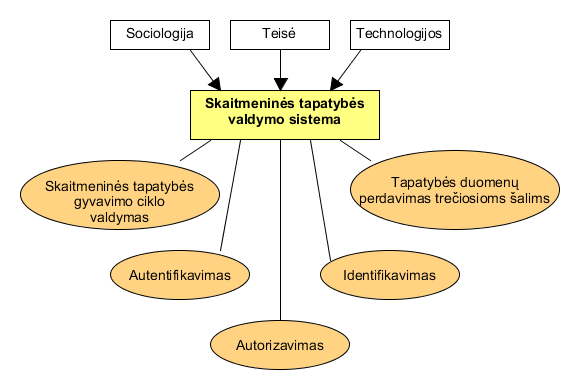
\includegraphics[scale=0.8]{img/IDMcontextAndUsecases}
    \caption{Skaitmeninių tapatybių valdymo sistemų kontekstas ir užduotys \cite{Glasser2009}}
\end{figure}

Paveiksle matomos disciplinos turi skirtingą poveikį tapatybių valdymo sistemoms. 
Sociologija padeda apibrėžti tapatybę ir jos atitikmenį skaitmeninėje erdvėje, teisės mokslas nusako tapatybės duomenų naudojimo reikalavimus,
o esamos technologijos formuoja sistemos įgyvendinimo niuansus. Verta pastebėti, kad tapatybės valdymo sistema gali atlikti ne visas
diagramoje nurodomas funkcijas, o tik dalį iš jų. Taip pat, 1-ame paveiksle bei visame darbe naudojamos skaitmeninės tapatybės valdymo sąvokos,
tokios kaip \textit{identifikavimas}, \textit{autentifikavimas} ar \textit{autorizavimas} neretai suprantamos skirtingai, o tai sukelia
vieningos terminologijos trūkumą ir dėl jo kylančius neaiškumus \cite{Glasser2009}. Dėl to skyriuje
\enquote{Sąvokų apibrėžimai} pateikiami darbe dažniausiai naudojamų terminų aiškinimai.

Esamų tapatybių valdymo sistemų architektūros bei veikimo principai yra skirtingi -  S. Clauß ir M.Köhntopp savo tyrime pastebi,
kad nėra vieningo standarto identiteto
valdymo sistemoms \cite{Claus2001}. Tolesniuose skyriuose, apžvelgus naudotojų bei paslaugų tiekėjų reikalavimus
tapatybės valdymo sistemoms, pateikiamos skirtingos technologijos
bei sprendimai, naudojami identiteto valdymui internete, jų privalumai bei trūkumai.

\subsection{Skaitmeninės tapatybės valdymo sistemų charakteristikos}

Skaitmeninės tapatybės valdymas yra plati sritis, kurią galima analizuoti iš skirtingų pusių.
Šiame darbe į skaitmeninių tapatybių valdymą žvelgta iš dviejų perspektyvų: naudotojo bei paslaugų tiekėjo \textcolor{red}{palikt tik naudotojo?}. Abi pusės,
priklausomai nuo savo poreikių, turi jiems aktualias identiteto valdymo sistemų savybes. Apžvelgiant skirtingas tapatybės valdymo sistemas,
didžiausias dėmėsys kreiptas į naudotojams bei paslaugų tiekėjams svarbiausius sistemų bruožus.

Tiek naudotojams, tiek paslaugų tiekėjams itin svarbus yra pasirinkto identiteto valdymo sprendimo patikimumas, t.y., asmens duomenų saugumo užtikrinimas.
Naudotojai nenori savo asmens duomenų nutekėjimo (angl. \textit{data leakage}) internete, tuo tarpu paslaugų tiekėjai negali rizikuoti prarasti naudotojų pasitikėjimo
jų paslauga pasirinkus nesaugų tapatybės valdymo sprendimą. Be patikimumo, naudotojams bei paslaugų tiekėjams aktualios ir 
kitos skaitmeninio identiteto sistemų savybės. Žemiau pateikiami pagrindiniai abiejų pusių poreikiai.
\\

\chapter{\textbf{Naudotojams svarbūs tapatybės valdymo sistemų bruožai:}}

\begin{itemize}
    \item identifikatorių bei slaptažodžių kiekis. Naudotojui vidutiniškai turint 25 paskyras, reikalaujančias slaptažodžių \cite{Florencio2007} bei naudojant
    nuo 2 iki 12-os el. paštų \cite{Gross2007}, jis tampa priverstas prisiminti vis daugiau identifikatorių. Atsimintinų autentifikavimo duomenų kiekiui
    augant, naudotojai yra linkę aukoti saugumą dėl patogumo ir naudoti panašius
    slaptažodžius skirtingose sistemose \cite{Pashalidis2003, Samar1999};
    \item asmens duomenų kontrolė. Pasak Nyderlanduose atliktų tyrimų, naudotojai jaučia, kad nekontroliuoja savo asmens duomenų internete \cite{Baars2016}. Dėl to
    naudotojai pradeda nepasitikėti taikomųjų programų kūrėjais, nes jie pilnai nežino, kokia informacija apie juos kaupiama ir kokioms
    sistemoms ji perduodama;
    \item patogumas (angl. \textit{usability}). Naudotojams skaitmeninės tapatybės valdymas dažnai yra tik pašalinis mechanizmas, reikalingas
    norint pasiekti paslaugą \cite{Dhamija2008}. Dėl šios priežasties sistemos naudojimosi patogumas yra svarbus - kuo tapatybės valdymas yra labiau integruotas
    su asmens jau naudojamomis sistemomis ir kuo mažiau jis reikalauja papildomo naudotojo įsitraukimo, tuo labiau naudotojas bus linkęs pasirinkti šį identiteto valdymo sprendimą.
\end{itemize}

\chapter{\textbf{Paslaugų tiekėjams aktualios tapatybės valdymo sistemų savybės:}}

\begin{itemize}
    \item kaštai, skirti tapatybės valdymui. Priklausomai nuo pasirinkto sprendimo,
    paslaugų tiekėjui gali tekti skirti daug arba mažai resursų (programuotojų, laiko, investavimo į technologijas)
    naudotojų tapatybės valdymo veiksmams užtikrinti;
    \item naudotojo patirties kontrolė (angl. \textit{user experience control}). Paslaugų tiekėjai siekia užtikrinti teigiamą
    naudotojų patirtį dėl geresnio naudojamumo, privatumo ir saugumo \cite{Dhamija2008}, o tapatybės valdymo sistemos veikimo primesti sprendimai (pvz. nukreipimai į kitą tinklalapį) gali daryti
    tam įtaką.
\end{itemize}

\subsection{Esamos skaitmeninių tapatybių valdymo sistemos}

Skirtingos tapatybių valdymo sistemos yra pagrįstos skirtingomis architektūromis, kurios įgalina
konkrečios sistemos veikimą. Šiame skyriuje apžvelgiami 3-ys dažniausiai naudojami tapatybių valdymo sistemų
modeliai bei pateikiami jų įgyvendinimo pavyzdžiai.

\subsubsection{Izoliuotas tapatybių valdymas}

\subsubsubsection*{Modelis}

Izoliuotame modelyje paslaugų tiekėjas yra ir tapatybės tiekėjas, nes visos su tapatybės valdymu
susijusios operacijos yra atliekamos vieno serverio. Tapatybės duomenų saugojimas, autentifikavimas
ir autorizavimas yra įgyvendinti paties paslaugų tiekėjo \cite{Cao2010} Kiekvienas naudotojas turi atskirus identifikatorius
kiekvienam paslaugų tiekėjui. Modelis grafiškai pavaizduotas žemiau esančiame paveiksle:

\begin{figure}[H]
    \centering
    \includegraphics[scale=0.65]{img/IsolatedModel}
    \caption{Izoliuotas skaitmeninės tapatybės valdymas \cite{Cao2010}}
\end{figure}

Pagal izoliuotą modelį, naudotojas turi savo paskyrą kiekvieno jam aktualaus paslaugų tiekėjo sistemoje. Kiekvieną kartą autentifikuojat ar autorizuojant
naudotoją, tai atlieka pats paslaugų tiekėjas, bendraudamas tiesiogiai su naudotoju (jo naršykle). Naudotojui prisijungus prie vieno tinklalapio ir gavus
prieigos raktą, jis gali toliau naudotis tinklalapiu, tačiau prireikus pasinaudoti kitu paslaugų tiekėju, tapatybės atpažinimo veiksmai (autentifikavimas, autorizavimas)
turės būti atlikti iš naujo su šiuo paslaugų tiekėju.

Šis modelis yra gana paprastas paslaugų tiekėjams, tačiau greitai tampa
nebekontroliuojamu naudotojams \cite{Josang2005}. Jis verčia naudotojus turėti daug paskyrų, identifikatorių bei slaptažodžių.
Tie patys tapatybės atpažinimo veiksmai (pvz. autentifikavimas) atliekamas iš naujo su kiekviena reikalinga paslauga. Naudotojui
sunku kontroliuoti savo asmens duomenis, nes jis juos patiki visiems paslaugų tiekėjams, kuriais naudojasi - tai apsunkina 
priežiūrą, kur kokie duomenys perduoti bei asmens duomenų atnaujinimą, kuris turi būti atliekamas su kiekvienu paslaugos tiekėju atskirai.

\textcolor{red}{jei reik, pastraipa paslaugų tiekėjo bruožams}.

\subsubsubsection*{Realizacijos}

Kadangi šis naudotojų autentifikavimo bei autorizavimo modelis naudojamas seniausiai,
yra gana nemažai jį įgyvendinusių taikomųjų programų. Lietuvoje šį modelį naudoja
\enquote{Tiketa}, \enquote{Bilietai.lt}, \enquote{Pigu.lt},
\enquote{Varle.lt}, pasaulyje - \enquote{Booking.com}, \enquote{Skycop}, \enquote{AirBnB} bei kitos platformos. Verta
pastebėti, kad dalis iš jų jau remiasi ne tik savo tapatybės valdymo, bet jau turi į savo sistemas integravę ir papildomų autentifikavimo būdų
(pvz. prisijungimą per \enquote{Facebook} ar \enquote{Google}).

Realizacijų technologiniai sprendimai dažniausiai nėra viešai prieinami.
Šiame modelyje kiekvienas paslaugų tiekėjas yra ir tapatybės tiekėjas, tad nereikia
specialaus protokolo, kuriuo duomenimis apsikeistų šios dvi esybės - visa tai pats nusprendžia
ir įgyvendina paslaugų tiekėjas.

\subsubsection{Centralizuotas tapatybių valdymas}

\subsubsubsection*{Modelis}
Centralizuotame skaitmeninių tapatybių valdyme egzistuoja vienas naudotojo identifikatorius,
naudojamas visų paslaugų tiekėjų \cite{Josang2005}. Paslaugų tiekėjo ir tapatybės tiekėjo funkcijos tampa atskirtos - 
tapatybės tiekėjas rūpinasi naudotojo identiteto valdymu, o paslaugų tiekėjas koncentruojasi į savo paslaugos tobulinimą.
Naudotojui šiame modelyje užtenka vieno identifikatoriaus ir slaptažodžio, su kuriais jis gali prisijungti prie visų to paties
paslaugų tiekėjo paslaugų. Šis modelis iliustruotas ~\ref{fig:isolatedModel}-iame paveiksle.

Iš naudotojo perspektyvos, šis modelis yra patogesnis nei izoliuotas. Naudotojui pakanka turėti vieną identifikatorių,
kuris bus tinkamas visoms paslaugoms. Priklausomai nuo realizacijos, naudotojui gali tekti iš naujo prisijungti prie kiekvienos
paslaugos arba vieną kartą prisijungti prie betkurios iš paslaugų ir tapti autentifikuotu visose kitose paslaugose \cite{Josang2005}. Naudotojo asmens
duomenų kontrolė yra geresnė nei izoliuotame skaitmeninės tapatybės valdyme, nes naudotojas asmens duomenis patiki mažesniam kiekiui esybių
(vietoj kiekvienos paslaugos, kiekvienam paslaugų tiekėjui).

Pagrindinis šio modelio trūkumas yra tas, kad jis galimas naudoti tik vieno paslaugų tiekėjo srityje (angl. \textit{scope}). Tai palieka laisvės paslaugų tiekėjui tapatybės valdymo sistemos
realizavimui (tai gali būti centralizuota platforma įmonės ribose), tačiau naudotojas negali turimo identifikatoriaus
naudoti kito paslaugų tiekėjo sistemose.

\begin{figure}[H]
    \centering
    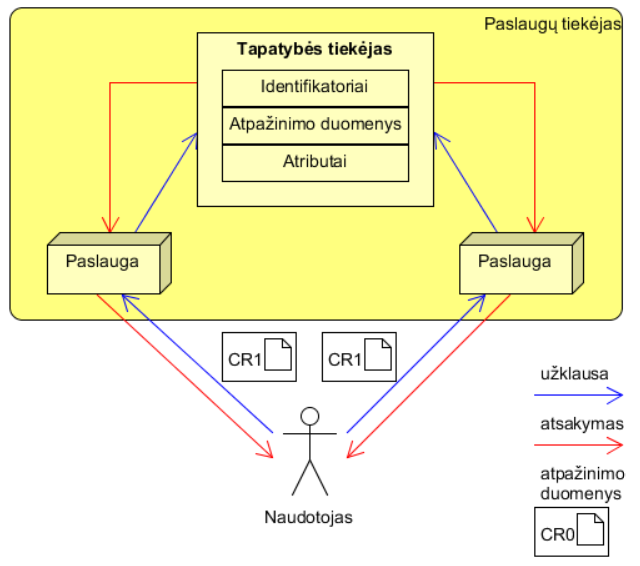
\includegraphics[scale=0.8]{img/centralizedModel}
    \caption{Centralizuotas skaitmeninės tapatybės valdymas \cite{Cao2010}}
    \label{fig:isolatedModel}
\end{figure}

\textcolor{red}{jei reik, pastraipa paslaugų tiekėjo bruožams}.

\subsubsubsection*{Realizacijos}

Centralizuotas modelis tinkamas naudoti vieno paslaugų tiekėjo ribose \cite{Josang2005}. Vienas iš pavyzdžių - 
\enquote{Atlassian} įmonės paslaugos. Naudotojui pakanka turėti vieną \enquote{Atlassian} paskyrą ir jis gali naudotis
skirtingais šio paslaugų tiekėjo produktais, tokiais kaip \enquote{Jira}, \enquote{Confluence}, \enquote{Bitbucket} bei kitais. \enquote{Atlassian}
turi ir vienkartinio prisijungimo sąlygas - paslaugas galima sukonfigūruoti taip, kad prisijungus prie vienos iš jų,
naudotojas automatiškai tampa prisijungęs ir prie kitų paslaugų.

Realizacijų naudojamos technologijos nėra viešai skelbiamos. Kadangi centralizuotame modelyje paslaugų tiekėjas
pats įgyvendina tapatybės tiekėjo modulį, jis pats apsprendžia bendravimą tarp tapatybės ir paslaugų tiekėjo. Priklausomai
nuo skirtingų paslaugų dydžio ir reikmių, šis bendravimas su tapatybės tiekėju gali svyruoti nuo centralizuotos duomenų bazės
naudotojų duomenims iki
paskirstytame tapatybės valdyme naudojamų technologijų (SAML, OpenID).

\subsubsection{Jungtinis tapatybių valdymas}

\subsubsubsection*{Modelis}

Centralizuotas modelis reikalauja visų naudotojų būti tame pačiame domene, tačiau naudotojams reikia
paslaugų ir iš kitų domenų \cite{Cao2010}. Jungtinis (angl. \textit{federated}) tapatybių valdymas yra aibė technologijų
ir procesų, kurie leidžia sistemoms dalintis tapatybės informacija ir deleguoti tapatybės valdymo užduotis
tarp skirtingų paslaugų tiekėjų \cite{Maler2008}. Šis tapatybių valdymo modelis įgalina naudotojus turėti vieną
identifikatorių, kurį gali naudoti skirtingų paslaugų tiekėjų tinklalapiuose. Žemiau pateikiama schema, nusakanti
šio modelio architektūrą:

\begin{figure}[H]
    \centering
    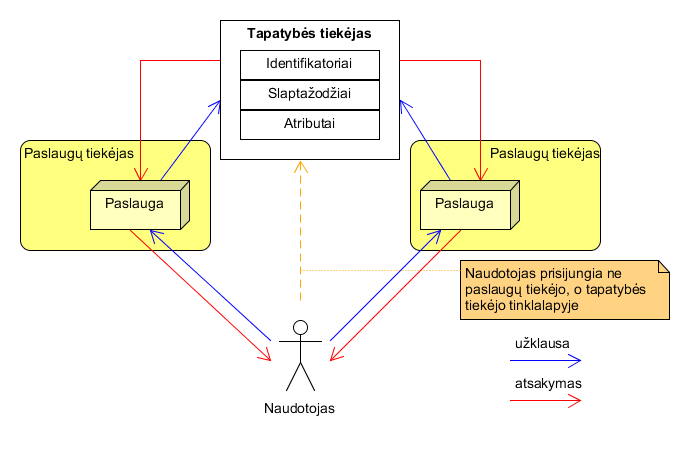
\includegraphics[scale=0.75]{img/federatedModel}
    \caption{Jungtinis skaitmeninės tapatybės valdymas \cite{Cao2010}}
    \label{fig:federatedModel}
\end{figure}

Jungtiniame tapatybės valdyme tapatybės tiekėjas yra atskira sistema, su kuria turi integruotis paslaugų tiekėjas. Tapatybės
duomenys bei su tapatybe susiję veiksmai (autentifikavimas, autorizavimas) yra deleguojami šiai sistemai. Naudotojas turi vieną identifikatorių,
su kuriuo prisijungia tiesiogiai tapatybės tiekėjo puslapyje. Prisijungus šioje sistemoje, naudotojas tampa
autentifikuotas visose paslaugose, kurios palaiko šį tapatybės tiekėją \cite{Maler2008}.

Šis tapatybių valdymo modelis yra gana patogus naudotojams. Jiems užtenka turėti vieną identifikatorių, su kuriuo
gali prisijungti prie tinklalapių iš skirtingų paslaugų tiekėjų. Asmens duomenų saugumas priklauso nuo
bendravimo tarp paslaugų bei tapatybės tiekėjų, o šiame modelyje jis sudėtingesnis nei izoliuotame ar centralizuotame
tapatybių valdyme, nes jungtinis valdymas paremtas tarpdomeniniu bendravimu \cite{Maler2008}. Naudotojo duomenų kontrolė jungtiniame 
modelyje turi tiek privalumų, tiek trūkumų. Viena vertus, naudotojas savo asmens duomenis suteikia mažesniam kiekiui sistemų (tik tapatybės tiekėjams,
vietoj visų paslaugų tiekėjų). Tačiau taip paslaugų tiekėjas tampa vieninteliu nesekmės tašku (angl. \textit{single point of failure}) - programišiams įsilaužus
į tapatybės tiekėjo sistemą, asmens paskyros visose paslaugose tampa prieinamos \cite{Pashalidis2003}. Taip pat, naudotojui gali būti sunku kontroliuoti
savo duomenų sklaidą tarp tapatybės tiekėjo ir skirtingų paslaugų, ką rodo ir \textit{Cambridge Analytica} incidentas \cite{CambridgeAnalytica}.

\textcolor{red}{jei reik, pastraipa paslaugų tiekėjo bruožams}.

\subsubsubsection*{Realizacijos}

\textcolor{red}{to be added}

\subsection{Tapatybių valdymo sistemų palyginimas}

% Please add the following required packages to your document preamble:
% \usepackage{multirow}
% \usepackage{graphicx}
\begin{table}[h]
    \centering
    \caption{My caption}
    \label{my-label}
    \resizebox{\textwidth}{!}{%
    \begin{tabular}{|l|l|l|l|l|l|}
    \hline
    \multicolumn{1}{|c|}{\multirow{2}{*}{Modelis}} & \multicolumn{1}{c|}{\multirow{2}{*}{\begin{tabular}[c]{@{}c@{}}Identifikatorių\\ kiekis\end{tabular}}} & \multicolumn{3}{c|}{Patogumas} & \multicolumn{1}{c|}{\multirow{2}{*}{\begin{tabular}[c]{@{}c@{}}Asmens duomenų\\ kontrolė\end{tabular}}} \\ \cline{3-5}
    \multicolumn{1}{|c|}{} & \multicolumn{1}{c|}{} & \multicolumn{1}{c|}{\begin{tabular}[c]{@{}c@{}}Prisijungimų\\ kiekis\end{tabular}} & \multicolumn{1}{c|}{\begin{tabular}[c]{@{}c@{}}Papildoma programinė\\ įranga\end{tabular}} & \multicolumn{1}{c|}{Naudotojo patirtis} & \multicolumn{1}{c|}{} \\ \hline
    Izoliuotas &  &  &  &  &  \\ \hline
    Centralizuotas &  &  &  &  &  \\ \hline
    Jungtinis &  &  &  &  &  \\ \hline
    \end{tabular}%
    }
    \end{table}

\sectionnonum{Rezultatai ir išvados}

\printbibliography[heading=bibintoc] 

\sectionnonum{Sąvokų apibrėžimai}
\textbf{Atributas} - charakteristika, susieta su esybe, pavyzdžiui fiziniu asmeniu. Galimi asmens atributai: gimimo data,
vardas, ūgis, pirštų antspaudai \cite{Camp2004}. Atributas gali būti laikinas (pvz. adresas) arba nuolatinis (pvz. asmens kodas).

\textbf{Identifikatorius} - tai atributas, kuris vienareikšmiškai susiejamas su jį pateikiančiu asmeniu ir kurį
sunku arba neįmanoma pakeisti. Fizinio asmens identifikatoriaus pavyzdys galėtų būti gimimo data
(žmogus gali apie ją meluoti, tačiau gimimo datos pakeisti neįmanoma) \cite{Camp2004}. Skaitmeninio identifikatoriaus
pavyzdys yra naudotojo elektroninio pašto adresas.

\textbf{Identifikavimas} - tai procesas, kurio metu asmuo susiejamas su jo identifikatoriumi \cite{Camp2004}. Identifikavimo
pavyzdys yra asmens ir jo vardo susiejimas: \textit{tu esi Jonas Jonaitis}.

\textbf{Autentifikavimas} - tai procesas, kurio metu patvirtinama sąsaja tarp tapatybės ir jos identifikatoriaus (t.y., įrodoma,
kad asmuo iš tikrųjų yra tas, kas sakosi esąs) \cite{Camp2004, Strictest2011}. Dažniausiai internete autentifikavimui pateikiamas identifikatorius
(pvz. slapyvardis) bei slaptažodis, susietas su tuo identifikatoriumi. Autentifikavimo pavyzdys:
\textit{tavo pateikta slapyvardžio ir slaptažodžio pora patvirtina, kad tu esi Jonas Jonaitis}.

\textbf{Autorizavimas} - tai procesas, kurio metu leidžiama arba draudžiama asmeniui atlikti konkretų veiksmą, priklausomai
nuo jo identifikatoriaus ar atributo \cite{Camp2004}. Pavyzdys: \textit{kadangi tau yra daugiau nei 18 metų, tu gali nusipirkti
energetinį gėrimą}. 

\textbf{Skaitmeninė tapatybė} - abstrakti fizinės esybės reprezentacija, sudaryta iš aibės esybės nuolatinių ar laikinų atributų,
kurie susiejami su fizine esybe \cite{Glasser2009, Camp2004}. Fizinė esybė gali būti fizinis arba juridinis asmuo.
Šiame darbe, jei nenurodyta kitaip, kalbama apie fizinio asmens skaitmeninę tapatybę.

\textbf{Skaitmeninės tapatybės valdymas} (angl. \textit{digital identity management}) - tai veiksmų, skirtų kontroliuoti
tapatybę ir su ja susijusius procesus, visuma \cite{Dabrowski2008}. Į tai įeina autentifikavimas, autorizavimas,
prieigų kontrolė, tapatybės gyvavimo ciklo
valdymas bei saugus tapatybės atributų perdavimas trečiosioms šalims \cite{Cao2010}.

\textbf{Skaitmeninių tapatybių domenas} - tai sritis, kurioje kiekviena tapatybė yra unikali. Domene esantys unikalūs
identifikatoriai leidžia sukurti vienas-su-vienu ryšį tarp šių identifikatorių ir jų tapatybių bei taip vienareikšmiškai
identifikuoti tapatybę iš jos unikalaus identifikatoriaus \cite{Josang2005}.

\textbf{Paslaugų tiekėjas} (angl. \textit{service provider}) - tai betkokia taikomoji programa, kuri suteikia naudotojui tam tikrą paslaugą ar
norimą turinį. Galimi paslaugų tiekėjai yra interneto tinklapiai, susirašinėjimo programos ar kitos taikomosios programos,
į kurias kreipiasi naudotojas \cite{Pashalidis2003, Samar1999}. Paslaugų tiekėjas gali turėti vieną ar kelias paslaugas,
kurioms reikia tapatybės valdymo funkcijų.

\textbf{Tapatybės tiekėjas} (angl. \textit{identity provider}) - servisas ar taikomoji programa, skirta koordinuoti su tapatybe
susijusius duomenis tarp naudotojų, jų naršyklių bei paslaugų tiekėjų \cite{Strictest2011}. Pagrindinės tapatybės tiekėjo funkcijos:
infrastruktūros naudotojų tapatybės duomenims apdoroti sukūrimas ir užklausų iš paslaugų tiekėjų bei naudotojų apdorojimas \cite{Cao2010}.

\textbf{Prieigos raktas} (angl. \textit{token}) - tai objektas, identifikuojantis skaitmeninę tapatybę \cite{TokenDefinition}.
Šis raktas būna išduodamas tapatybės tiekėjo ir skirtas identifikuoti naudotoją. Raktas
būna prisegtas prie visų autentifikuoto naudotojo užklausų ir leidžia paslaugos tiekėjui žinoti, koks naudotojas kreipiasi.

\textbf{Vienkartinis prisijungimas} (angl. \textit{single sign on}) - \textcolor{red}{to be added}.

\end{document}